\documentclass[twoside]{book}

% Packages required by doxygen
\usepackage{fixltx2e}
\usepackage{calc}
\usepackage{doxygen}
\usepackage[export]{adjustbox} % also loads graphicx
\usepackage{graphicx}
\usepackage[utf8]{inputenc}
\usepackage{makeidx}
\usepackage{multicol}
\usepackage{multirow}
\PassOptionsToPackage{warn}{textcomp}
\usepackage{textcomp}
\usepackage[nointegrals]{wasysym}
\usepackage[table]{xcolor}

% Font selection
\usepackage[T1]{fontenc}
\usepackage[scaled=.90]{helvet}
\usepackage{courier}
\usepackage{amssymb}
\usepackage{sectsty}
\renewcommand{\familydefault}{\sfdefault}
\allsectionsfont{%
  \fontseries{bc}\selectfont%
  \color{darkgray}%
}
\renewcommand{\DoxyLabelFont}{%
  \fontseries{bc}\selectfont%
  \color{darkgray}%
}
\newcommand{\+}{\discretionary{\mbox{\scriptsize$\hookleftarrow$}}{}{}}

% Page & text layout
\usepackage{geometry}
\geometry{%
  a4paper,%
  top=2.5cm,%
  bottom=2.5cm,%
  left=2.5cm,%
  right=2.5cm%
}
\tolerance=750
\hfuzz=15pt
\hbadness=750
\setlength{\emergencystretch}{15pt}
\setlength{\parindent}{0cm}
\setlength{\parskip}{3ex plus 2ex minus 2ex}
\makeatletter
\renewcommand{\paragraph}{%
  \@startsection{paragraph}{4}{0ex}{-1.0ex}{1.0ex}{%
    \normalfont\normalsize\bfseries\SS@parafont%
  }%
}
\renewcommand{\subparagraph}{%
  \@startsection{subparagraph}{5}{0ex}{-1.0ex}{1.0ex}{%
    \normalfont\normalsize\bfseries\SS@subparafont%
  }%
}
\makeatother

% Headers & footers
\usepackage{fancyhdr}
\pagestyle{fancyplain}
\fancyhead[LE]{\fancyplain{}{\bfseries\thepage}}
\fancyhead[CE]{\fancyplain{}{}}
\fancyhead[RE]{\fancyplain{}{\bfseries\leftmark}}
\fancyhead[LO]{\fancyplain{}{\bfseries\rightmark}}
\fancyhead[CO]{\fancyplain{}{}}
\fancyhead[RO]{\fancyplain{}{\bfseries\thepage}}
\fancyfoot[LE]{\fancyplain{}{}}
\fancyfoot[CE]{\fancyplain{}{}}
\fancyfoot[RE]{\fancyplain{}{\bfseries\scriptsize Generated by Doxygen }}
\fancyfoot[LO]{\fancyplain{}{\bfseries\scriptsize Generated by Doxygen }}
\fancyfoot[CO]{\fancyplain{}{}}
\fancyfoot[RO]{\fancyplain{}{}}
\renewcommand{\footrulewidth}{0.4pt}
\renewcommand{\chaptermark}[1]{%
  \markboth{#1}{}%
}
\renewcommand{\sectionmark}[1]{%
  \markright{\thesection\ #1}%
}

% Indices & bibliography
\usepackage{natbib}
\usepackage[titles]{tocloft}
\setcounter{tocdepth}{3}
\setcounter{secnumdepth}{5}
\makeindex

% Custom commands
\newcommand{\clearemptydoublepage}{%
  \newpage{\pagestyle{empty}\cleardoublepage}%
}

\usepackage{caption}
\captionsetup{labelsep=space,justification=centering,font={bf},singlelinecheck=off,skip=4pt,position=top}

%===== C O N T E N T S =====

\begin{document}

% Titlepage & ToC
\pagenumbering{alph}
\begin{titlepage}
\vspace*{7cm}
\begin{center}%
{\Large Software documentation -\/ Command-\/line tools W\+F\+YD }\\
\vspace*{1cm}
{\large Generated by Doxygen 1.8.13}\\
\end{center}
\end{titlepage}
\clearemptydoublepage
\pagenumbering{roman}
\tableofcontents
\clearemptydoublepage
\pagenumbering{arabic}

%--- Begin generated contents ---
\chapter{Command line tools}
\label{index}This is the firmware of W\+F\+YD. \begin{DoxyVersion}{Version}
1.\+0
\end{DoxyVersion}
This is the firmware of the W\+F\+YD. It can control two motors and a servo motors and read their encoders. Also can read and convert analog measurements connected to the P\+SoC microcontroller. 
\chapter{Data Structure Index}
\section{Data Structures}
Here are the data structures with brief descriptions\+:\begin{DoxyCompactList}
\item\contentsline{section}{\textbf{ st\+\_\+data} }{\pageref{structst__data}}{}
\item\contentsline{section}{\textbf{ st\+\_\+meas} }{\pageref{structst__meas}}{}
\item\contentsline{section}{\textbf{ st\+\_\+mem} }{\pageref{structst__mem}}{}
\item\contentsline{section}{\textbf{ st\+\_\+ref} }{\pageref{structst__ref}}{}
\end{DoxyCompactList}

\chapter{File Index}
\section{File List}
Here is a list of all documented files with brief descriptions\+:\begin{DoxyCompactList}
\item\contentsline{section}{\textbf{ command\+\_\+processing.\+c} \\*Command processing functions }{\pageref{command__processing_8c}}{}
\item\contentsline{section}{\textbf{ command\+\_\+processing.\+h} \\*Command processing functions }{\pageref{command__processing_8h}}{}
\item\contentsline{section}{\textbf{ commands.\+h} \\*Definitions for commands, parameters and packages }{\pageref{commands_8h}}{}
\item\contentsline{section}{{\bfseries device.\+h} }{\pageref{device_8h}}{}
\item\contentsline{section}{\textbf{ globals.\+c} \\*Global variables }{\pageref{globals_8c}}{}
\item\contentsline{section}{\textbf{ globals.\+h} \\*Global definitions and macros are set in this file }{\pageref{globals_8h}}{}
\item\contentsline{section}{\textbf{ interruptions.\+c} \\*Interruption functions are in this file }{\pageref{interruptions_8c}}{}
\item\contentsline{section}{\textbf{ interruptions.\+h} \\*Interruptions header file }{\pageref{interruptions_8h}}{}
\item\contentsline{section}{\textbf{ main.\+c} \\*Firmware main file }{\pageref{main_8c}}{}
\item\contentsline{section}{\textbf{ utils.\+h} \\*Definition of utility functions }{\pageref{utils_8h}}{}
\end{DoxyCompactList}

\chapter{Data Structure Documentation}
\section{global\+\_\+args Struct Reference}
\label{structglobal__args}\index{global\+\_\+args@{global\+\_\+args}}
\subsection*{Data Fields}
\begin{DoxyCompactItemize}
\item 
\mbox{\label{structglobal__args_accfd0301c469314772cc651ec198d492}} 
int {\bfseries device\+\_\+id}
\item 
\mbox{\label{structglobal__args_a8c2bd6bbe7e544186ac9dafe368eda0a}} 
int \textbf{ flag\+\_\+set\+\_\+inputs}
\begin{DoxyCompactList}\small\item\em ./qbmove -\/s option \end{DoxyCompactList}\item 
\mbox{\label{structglobal__args_ae6be84e61dfa72e2992e18b2ff872d37}} 
int \textbf{ flag\+\_\+get\+\_\+measurements}
\begin{DoxyCompactList}\small\item\em ./qbmove -\/g option \end{DoxyCompactList}\item 
\mbox{\label{structglobal__args_a357acdae444e13e67d3747246a2a6537}} 
int \textbf{ flag\+\_\+activate}
\begin{DoxyCompactList}\small\item\em ./qbmove -\/a option \end{DoxyCompactList}\item 
\mbox{\label{structglobal__args_a3f8a32491b8271e7dcf9645888fd5d90}} 
int \textbf{ flag\+\_\+deactivate}
\begin{DoxyCompactList}\small\item\em ./qbmove -\/d option \end{DoxyCompactList}\item 
\mbox{\label{structglobal__args_a666e67d4cbdc4b0c0ceaebc7f0d7e4ae}} 
int \textbf{ flag\+\_\+ping}
\begin{DoxyCompactList}\small\item\em ./qbmove -\/p option \end{DoxyCompactList}\item 
\mbox{\label{structglobal__args_a5d91f73cfac19063f3b690444214cb11}} 
int \textbf{ flag\+\_\+serial\+\_\+port}
\begin{DoxyCompactList}\small\item\em ./qbmove -\/t option \end{DoxyCompactList}\item 
\mbox{\label{structglobal__args_a2d410324c656ed3cf62239ef07f19df6}} 
int \textbf{ flag\+\_\+verbose}
\begin{DoxyCompactList}\small\item\em ./qbmove -\/v option \end{DoxyCompactList}\item 
\mbox{\label{structglobal__args_a66d5c9e9750727f229d685d9399218d0}} 
int \textbf{ flag\+\_\+set\+\_\+zeros}
\begin{DoxyCompactList}\small\item\em ./qbmove -\/z option \end{DoxyCompactList}\item 
\mbox{\label{structglobal__args_a884582f66057291a6a1f030d5d46d9d5}} 
int \textbf{ flag\+\_\+get\+\_\+currents}
\begin{DoxyCompactList}\small\item\em ./qbmove -\/c option \end{DoxyCompactList}\item 
\mbox{\label{structglobal__args_a8488439bc3473b5fb08964d06b51b80a}} 
int \textbf{ flag\+\_\+bootloader\+\_\+mode}
\begin{DoxyCompactList}\small\item\em ./qbmove -\/b option \end{DoxyCompactList}\item 
\mbox{\label{structglobal__args_aa9b8d91302ac6dbb99023c9363c352f8}} 
int \textbf{ flag\+\_\+get\+\_\+velocities}
\begin{DoxyCompactList}\small\item\em ./qbmove -\/i option \end{DoxyCompactList}\item 
\mbox{\label{structglobal__args_af72013af180143fd3cce334fca450bec}} 
int \textbf{ flag\+\_\+get\+\_\+accelerations}
\begin{DoxyCompactList}\small\item\em ./qbmove -\/o option \end{DoxyCompactList}\item 
\mbox{\label{structglobal__args_a24ec0f8144d1376bd72b06667b12b088}} 
int \textbf{ flag\+\_\+get\+\_\+ir}
\begin{DoxyCompactList}\small\item\em ./qbmove -\/I option \end{DoxyCompactList}\item 
\mbox{\label{structglobal__args_a3d4f1fdf9bfdbe27109015605252ff5c}} 
int \textbf{ flag\+\_\+set\+\_\+servo}
\begin{DoxyCompactList}\small\item\em ./qbmove -\/S option \end{DoxyCompactList}\item 
\mbox{\label{structglobal__args_a8e7f619fb332291848bceae1fef502f1}} 
int \textbf{ flag\+\_\+get\+\_\+servo}
\begin{DoxyCompactList}\small\item\em ./qbmove -\/G option \end{DoxyCompactList}\item 
\mbox{\label{structglobal__args_abda0b0b3f5ad08a7fe15bb29b5de123b}} 
int \textbf{ flag\+\_\+get\+\_\+force}
\begin{DoxyCompactList}\small\item\em ./qbmove -\/F option \end{DoxyCompactList}\item 
\mbox{\label{structglobal__args_ac6a0f577c519bd619725257c46c8e100}} 
int \textbf{ flag\+\_\+get\+\_\+duty}
\begin{DoxyCompactList}\small\item\em ./qbmove -\/D option \end{DoxyCompactList}\item 
\mbox{\label{structglobal__args_a6b371b126c5346f512bcb9f3700213c7}} 
int \textbf{ flag\+\_\+sinusoid}
\begin{DoxyCompactList}\small\item\em ./qbmove -\/N option \end{DoxyCompactList}\item 
\mbox{\label{structglobal__args_aeb7e77450221e7de1da5ae0701a8c7af}} 
int \textbf{ flag\+\_\+set\+\_\+baudrate}
\begin{DoxyCompactList}\small\item\em ./qbmove -\/R option \end{DoxyCompactList}\item 
\mbox{\label{structglobal__args_a5416bb93d203c57a7fc6fe93957f5c14}} 
int \textbf{ flag\+\_\+set\+\_\+watchdog}
\begin{DoxyCompactList}\small\item\em ./qbmove -\/W option \end{DoxyCompactList}\item 
\mbox{\label{structglobal__args_ab4fab167b07a819ebd9cdff9d9c232b0}} 
int \textbf{ flag\+\_\+polling}
\begin{DoxyCompactList}\small\item\em ./qbmove -\/P option \end{DoxyCompactList}\item 
\mbox{\label{structglobal__args_a9781d8e86f2d0d0414d313fec085d20e}} 
int \textbf{ flag\+\_\+baudrate}
\begin{DoxyCompactList}\small\item\em ./qbmove -\/B option \end{DoxyCompactList}\item 
\mbox{\label{structglobal__args_a5c5d83977377b63e3671b52680be11aa}} 
short int {\bfseries inputs} [N\+U\+M\+\_\+\+O\+F\+\_\+\+M\+O\+T\+O\+RS]
\item 
\mbox{\label{structglobal__args_a4c65d251aa919a9ae56d11639a748ccf}} 
short int {\bfseries measurements} [4]
\item 
\mbox{\label{structglobal__args_aa064f75f1bb48d252dabea993cd8c393}} 
short int {\bfseries velocities} [4]
\item 
\mbox{\label{structglobal__args_a6fe131122f89735be8fb030f8333e8c8}} 
short int {\bfseries accelerations} [4]
\item 
\mbox{\label{structglobal__args_a8e63e8b1dcf1ee3b6429110e26a7ef3d}} 
short int {\bfseries measurement\+\_\+offset} [4]
\item 
\mbox{\label{structglobal__args_aff0783d0bf2ae80eadc0c85a84db1549}} 
short int {\bfseries currents} [N\+U\+M\+\_\+\+O\+F\+\_\+\+M\+O\+T\+O\+RS]
\item 
\mbox{\label{structglobal__args_ad9b862535a2c85c9ca5f9b1b6f858f0e}} 
short int {\bfseries measurement\+\_\+ir} [1]
\item 
\mbox{\label{structglobal__args_a312ac8e2e59fa39822997368bdb4ad30}} 
short int {\bfseries measurement\+\_\+servo} [1]
\item 
\mbox{\label{structglobal__args_a47308e49ae17b1827646db852e731514}} 
short int {\bfseries inputservo} [1]
\item 
\mbox{\label{structglobal__args_ac5812e19901605235ea1a1fb8c79b695}} 
short int {\bfseries measurement\+\_\+force} [1]
\item 
\mbox{\label{structglobal__args_a7013a2c89b79b5e482f024f1eaa78b9b}} 
short int {\bfseries meas\+\_\+duty\+\_\+cy\+\_\+max} [1]
\item 
\mbox{\label{structglobal__args_a8f68c2db71004b2beac47c7ce6feb94c}} 
short int {\bfseries Baud\+Rate}
\item 
\mbox{\label{structglobal__args_a15a8bc4e37e5294ee939c1dd620095a8}} 
int {\bfseries save\+\_\+baurate}
\item 
\mbox{\label{structglobal__args_abd2a5fb7d2e58a98c4394067565b5492}} 
short int {\bfseries W\+DT}
\item 
\mbox{\label{structglobal__args_ac3ca959d3b7ae254f86531e0b82affcb}} 
F\+I\+LE $\ast$ {\bfseries emg\+\_\+file}
\item 
\mbox{\label{structglobal__args_a5fbba9db8f8d479d7607ec6e8617026a}} 
F\+I\+LE $\ast$ {\bfseries log\+\_\+file\+\_\+fd}
\end{DoxyCompactItemize}


The documentation for this struct was generated from the following file\+:\begin{DoxyCompactItemize}
\item 
\textbf{ qbadmin.\+c}\end{DoxyCompactItemize}

\section{position Struct Reference}
\label{structposition}\index{position@{position}}
\subsection*{Data Fields}
\begin{DoxyCompactItemize}
\item 
\mbox{\label{structposition_a3f6abbd70f28831ca50df1deece62d27}} 
float {\bfseries prec}
\item 
\mbox{\label{structposition_acd65ff39e6ad988e189dc854d5ede11b}} 
float {\bfseries act}
\end{DoxyCompactItemize}


The documentation for this struct was generated from the following file\+:\begin{DoxyCompactItemize}
\item 
\textbf{ qbadmin.\+c}\end{DoxyCompactItemize}

\chapter{File Documentation}
\section{definitions.\+h File Reference}
\label{definitions_8h}\index{definitions.\+h@{definitions.\+h}}


Definitions for board commands, parameters and packages.  


{\ttfamily \#include $<$math.\+h$>$}\newline
Include dependency graph for definitions.\+h\+:
\nopagebreak
\begin{figure}[H]
\begin{center}
\leavevmode
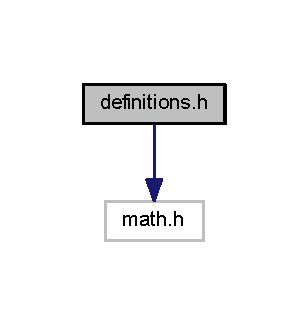
\includegraphics[width=148pt]{definitions_8h__incl}
\end{center}
\end{figure}
This graph shows which files directly or indirectly include this file\+:
\nopagebreak
\begin{figure}[H]
\begin{center}
\leavevmode
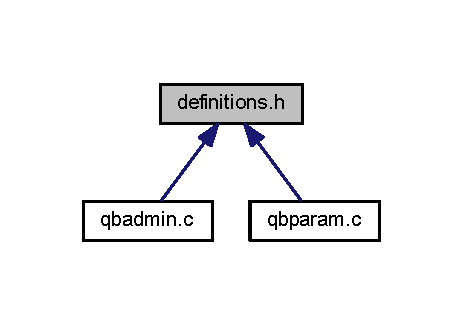
\includegraphics[width=222pt]{definitions_8h__dep__incl}
\end{center}
\end{figure}
\subsection*{Macros}
\begin{DoxyCompactItemize}
\item 
\mbox{\label{definitions_8h_a82178bde559e31158313c53e55709f7b}} 
\#define {\bfseries Q\+B\+A\+D\+M\+I\+N\+\_\+\+V\+E\+R\+S\+I\+ON}~\char`\"{}v6.\+1.\+0\char`\"{}
\item 
\mbox{\label{definitions_8h_a39ac50737c1ee7d5b723b2597fdf6f26}} 
\#define {\bfseries N\+U\+M\+\_\+\+O\+F\+\_\+\+M\+O\+T\+O\+RS}~2
\item 
\mbox{\label{definitions_8h_a8e55cba7b8d4f9aa1eb36f311ce121e5}} 
\#define {\bfseries N\+U\+M\+\_\+\+O\+F\+\_\+\+E\+M\+GS}~2
\item 
\mbox{\label{definitions_8h_a598a3330b3c21701223ee0ca14316eca}} 
\#define {\bfseries PI}~3.\+14159265359
\item 
\mbox{\label{definitions_8h_a2674041fcb6b33ea03b7441c5bf07da1}} 
\#define {\bfseries D\+E\+F\+A\+U\+L\+T\+\_\+\+R\+E\+S\+O\+L\+U\+T\+I\+ON}~1
\item 
\mbox{\label{definitions_8h_a9df8ee92f567229e4e969a89792f7909}} 
\#define {\bfseries D\+E\+F\+A\+U\+L\+T\+\_\+\+I\+N\+F\+\_\+\+L\+I\+M\+IT}~-\/15000
\item 
\mbox{\label{definitions_8h_a664de08cc70be246edd326c4832574bb}} 
\#define {\bfseries D\+E\+F\+A\+U\+L\+T\+\_\+\+S\+U\+P\+\_\+\+L\+I\+M\+IT}~15000
\item 
\mbox{\label{definitions_8h_ab9fe47395310b34fa1ceb112c9ca10e2}} 
\#define {\bfseries B\+R\+O\+A\+D\+C\+A\+S\+T\+\_\+\+ID}~0
\item 
\mbox{\label{definitions_8h_a4c6daad09923a0ab3ed52ebb1c0b8cb8}} 
\#define {\bfseries D\+E\+F\+A\+U\+L\+T\+\_\+\+P\+I\+D\+\_\+P}~0.\+1
\item 
\mbox{\label{definitions_8h_a6f7a63a5d40ee41381abe79b78993567}} 
\#define {\bfseries D\+E\+F\+A\+U\+L\+T\+\_\+\+P\+I\+D\+\_\+I}~0
\item 
\mbox{\label{definitions_8h_ab285c4cd42477c9669f9981d03572d2f}} 
\#define {\bfseries D\+E\+F\+A\+U\+L\+T\+\_\+\+P\+I\+D\+\_\+D}~0.\+8
\item 
\mbox{\label{definitions_8h_a4956377066b3b3074de9c79d7e1d8967}} 
\#define {\bfseries D\+E\+F\+A\+U\+L\+T\+\_\+\+I\+N\+C\+R\+E\+M\+E\+NT}~1
\item 
\mbox{\label{definitions_8h_a8c5790f774337ec087041124dda03ed4}} 
\#define {\bfseries D\+E\+F\+A\+U\+L\+T\+\_\+\+S\+T\+I\+F\+F\+N\+E\+SS}~30
\item 
\mbox{\label{definitions_8h_a92f641bf6a2b5f3e0277d62d29158bff}} 
\#define {\bfseries D\+E\+F\+A\+U\+L\+T\+\_\+\+M\+A\+X\+\_\+\+E\+X\+C\+U\+R\+S\+I\+ON}~330
\item 
\mbox{\label{definitions_8h_ac328e551bde3d39b6d7b8cc9e048d941}} 
\#define {\bfseries Z\+E\+RO}~0
\item 
\mbox{\label{definitions_8h_a2719be2b85fcfd6fd26291a9a7775ea7}} 
\#define {\bfseries M\+A\+X\+\_\+\+F\+O\+R\+W\+A\+R\+D\+\_\+\+S\+T\+I\+F\+F\+N\+E\+SS}~32767
\item 
\mbox{\label{definitions_8h_ad91fa28a852c573709249b16fca30d23}} 
\#define {\bfseries M\+A\+X\+\_\+\+R\+E\+V\+E\+R\+S\+E\+\_\+\+S\+T\+I\+F\+F\+N\+E\+SS}~-\/32768
\item 
\mbox{\label{definitions_8h_adc098850cdde5fbe8e5f4fe910f9ce27}} 
\#define {\bfseries D\+E\+G\+\_\+\+T\+I\+C\+K\+\_\+\+M\+U\+L\+T\+I\+P\+L\+I\+ER}~(65536.\+0 / (360.\+0 $\ast$ (pow(2, D\+E\+F\+A\+U\+L\+T\+\_\+\+R\+E\+S\+O\+L\+U\+T\+I\+ON))))
\item 
\mbox{\label{definitions_8h_a44483e681594d0e510fd59c2b4b09ed9}} 
\#define {\bfseries B\+A\+U\+D\+\_\+\+R\+A\+T\+E\+\_\+\+T\+\_\+2000000}~0
\item 
\mbox{\label{definitions_8h_ad2c3e3edb0886633d686996e2f8c48e6}} 
\#define {\bfseries B\+A\+U\+D\+\_\+\+R\+A\+T\+E\+\_\+\+T\+\_\+460800}~1
\item 
\mbox{\label{definitions_8h_a342ce09900d5e0dc2b6adb9afe5f1778}} 
\#define {\bfseries S\+I\+N\+\_\+\+F\+I\+LE}~\char`\"{}./../conf\+\_\+files/sin.\+conf\char`\"{}
\item 
\mbox{\label{definitions_8h_aaf3958c9ffdb0121b3ae603509e15d44}} 
\#define {\bfseries M\+O\+T\+O\+R\+\_\+\+F\+I\+LE}~\char`\"{}./../conf\+\_\+files/motor.\+conf\char`\"{}
\item 
\mbox{\label{definitions_8h_a85af9928ee1b7b3029d40a0058e617de}} 
\#define {\bfseries Q\+B\+M\+O\+V\+E\+\_\+\+F\+I\+LE}~\char`\"{}./../conf\+\_\+files/qbmove.\+conf\char`\"{}
\item 
\mbox{\label{definitions_8h_ad0c21fc604bc4dae8a306f330762b8b5}} 
\#define {\bfseries Q\+B\+B\+A\+C\+K\+U\+P\+\_\+\+F\+I\+LE}~\char`\"{}./../conf\+\_\+files/qbbackup.\+conf\char`\"{}
\item 
\mbox{\label{definitions_8h_a73d175f1cc3a063336277351cf7feb42}} 
\#define {\bfseries Q\+B\+M\+O\+V\+E\+\_\+\+F\+I\+L\+E\+\_\+\+BR}~\char`\"{}./../conf\+\_\+files/qbmove\+B\+R.\+conf\char`\"{}
\item 
\mbox{\label{definitions_8h_ab1563f614ecc2b82f97cd65b88217bd9}} 
\#define \textbf{ E\+M\+G\+\_\+\+S\+A\+V\+E\+D\+\_\+\+V\+A\+L\+U\+ES}~\char`\"{}./../emg\+\_\+values.\+csv\char`\"{}
\begin{DoxyCompactList}\small\item\em Default location where the emg sensors values are saved. \end{DoxyCompactList}\end{DoxyCompactItemize}


\subsection{Detailed Description}
Definitions for board commands, parameters and packages. 

\begin{DoxyAuthor}{Author}
{\itshape Centro \char`\"{}\+E.\+Piaggio\char`\"{}} 
\end{DoxyAuthor}
\begin{DoxyCopyright}{Copyright}
(C) 2012-\/2016 qbrobotics. All rights reserved. 

(C) 2017 Centro \char`\"{}\+E.\+Piaggio\char`\"{}. All rights reserved.
\end{DoxyCopyright}
This file is included in the board firmware, in its libraries and applications. It contains all definitions that are necessary for the contruction of communication packages.

It includes definitions for all of the device commands, parameters and also the size of answer packages. 
\section{qbadmin.\+c File Reference}
\label{qbadmin_8c}\index{qbadmin.\+c@{qbadmin.\+c}}


Command line tools file.  


{\ttfamily \#include \char`\"{}../../qb\+A\+P\+I/src/qbmove\+\_\+communications.\+h\char`\"{}}\newline
{\ttfamily \#include \char`\"{}../../qb\+A\+P\+I/src/w\+\_\+fyd\+\_\+communications.\+h\char`\"{}}\newline
{\ttfamily \#include \char`\"{}definitions.\+h\char`\"{}}\newline
{\ttfamily \#include $<$stdio.\+h$>$}\newline
{\ttfamily \#include $<$stdlib.\+h$>$}\newline
{\ttfamily \#include $<$unistd.\+h$>$}\newline
{\ttfamily \#include $<$getopt.\+h$>$}\newline
{\ttfamily \#include $<$string.\+h$>$}\newline
{\ttfamily \#include $<$sys/time.\+h$>$}\newline
{\ttfamily \#include $<$math.\+h$>$}\newline
{\ttfamily \#include $<$signal.\+h$>$}\newline
{\ttfamily \#include $<$assert.\+h$>$}\newline
Include dependency graph for qbadmin.\+c\+:
\nopagebreak
\begin{figure}[H]
\begin{center}
\leavevmode
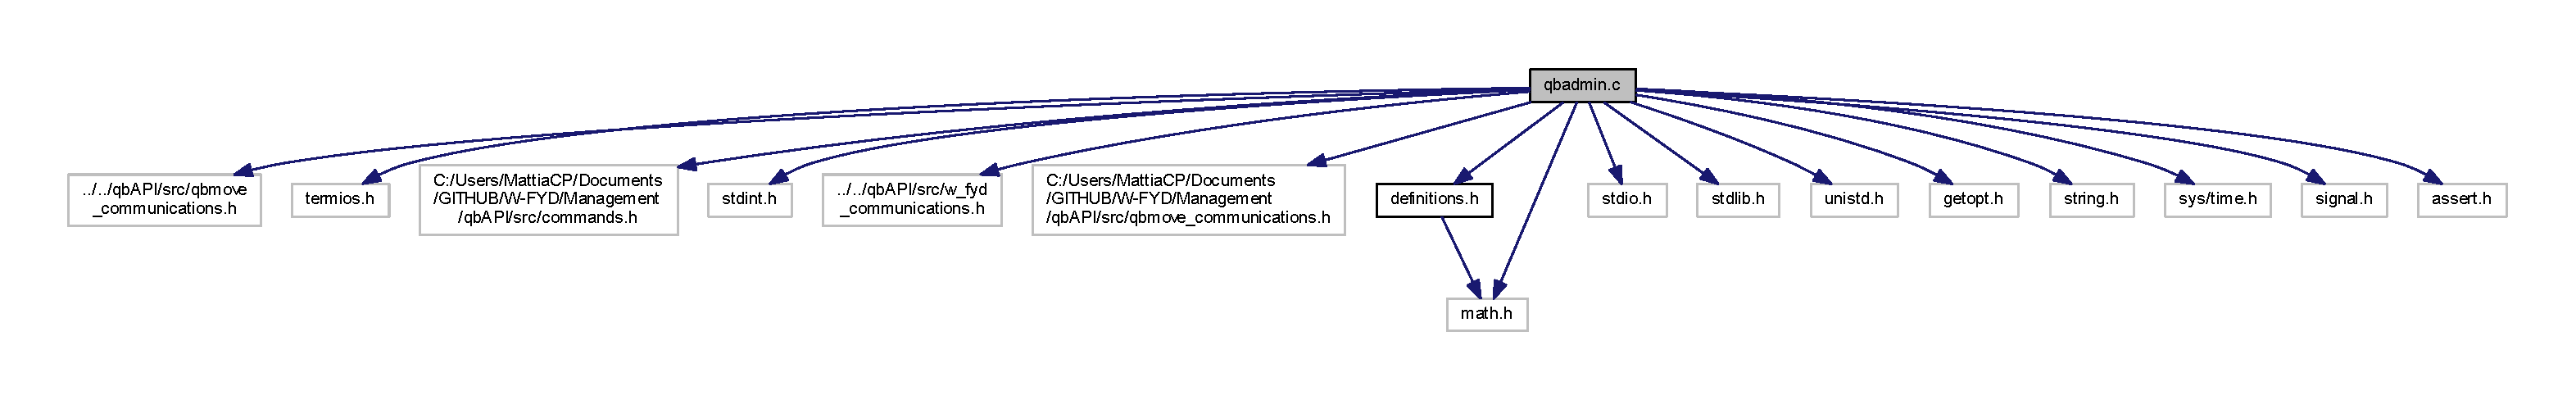
\includegraphics[width=350pt]{qbadmin_8c__incl}
\end{center}
\end{figure}
\subsection*{Data Structures}
\begin{DoxyCompactItemize}
\item 
struct \textbf{ global\+\_\+args}
\item 
struct \textbf{ position}
\end{DoxyCompactItemize}
\subsection*{Functions}
\begin{DoxyCompactItemize}
\item 
\mbox{\label{qbadmin_8c_abe553924eef0ba8079dc745caf1f348c}} 
int {\bfseries open\+\_\+port} ()
\item 
\mbox{\label{qbadmin_8c_a3939d4ef4a0e2be02b1eb9e1994ec985}} 
int {\bfseries port\+\_\+selection} ()
\item 
\mbox{\label{qbadmin_8c_a22b6aac07ec93fb920cc09b13175fa20}} 
int {\bfseries polling} ()
\item 
void \textbf{ display\+\_\+usage} (void)
\item 
float $\ast$$\ast$ \textbf{ file\+\_\+parser} (char $\ast$, int $\ast$, int $\ast$)
\item 
void \textbf{ int\+\_\+handler} (int sig)
\item 
void \textbf{ int\+\_\+handler\+\_\+2} (int sig)
\item 
void \textbf{ int\+\_\+handler\+\_\+3} (int sig)
\item 
int \textbf{ baudrate\+\_\+reader} ()
\item 
\mbox{\label{qbadmin_8c_abab28310fbbbcecb4658ce38e10ae89a}} 
int {\bfseries baudrate\+\_\+writer} (const int)
\item 
\mbox{\label{qbadmin_8c_aa13424f8e83a570e769decb4c02398d2}} 
double {\bfseries elapsed\+\_\+time} (S\+Y\+S\+T\+E\+M\+T\+I\+ME current, S\+Y\+S\+T\+E\+M\+T\+I\+ME reference)
\item 
int \textbf{ main} (int argc, char $\ast$$\ast$argv)
\end{DoxyCompactItemize}
\subsection*{Variables}
\begin{DoxyCompactItemize}
\item 
static const struct option {\bfseries long\+Opts} [$\,$]
\item 
\mbox{\label{qbadmin_8c_a1b7271ddd60c22960c39ae6caf4d5254}} 
static const char $\ast$ {\bfseries opt\+String} = \char`\"{}s\+:adgptvh?f\+:ljqxzkycbe\+:uoi\+W\+:\+P\+B\+:\+I\+S\+:\+G\+F\+DN\char`\"{}
\item 
\mbox{\label{qbadmin_8c_ac8e0866643ba994eff3e2fa3203885e0}} 
struct \textbf{ global\+\_\+args} {\bfseries global\+\_\+args}
\item 
\mbox{\label{qbadmin_8c_a821afb7ce4f1050e40bf615da3259a67}} 
struct \textbf{ position} {\bfseries p1}
\item 
\mbox{\label{qbadmin_8c_aeb1c5de60c0abd963c4b508d9f4c3cb1}} 
struct \textbf{ position} {\bfseries p2}
\item 
\mbox{\label{qbadmin_8c_a761d62937db066110a8f3e1479e8c404}} 
uint8\+\_\+t {\bfseries resolution} [4]
\item 
\mbox{\label{qbadmin_8c_a6baa346e44f4c2158d2be4f9b77b8203}} 
int {\bfseries ret}
\item 
\mbox{\label{qbadmin_8c_abf8643fca8c83efc67b50d0f2ecc8534}} 
int {\bfseries aux\+\_\+int}
\item 
\mbox{\label{qbadmin_8c_ae80455d5ff9aa4415b211f9842cb885e}} 
comm\+\_\+settings {\bfseries comm\+\_\+settings\+\_\+1}
\item 
\mbox{\label{qbadmin_8c_ab7561703ea7d6e95482c3c0aa4ce41bd}} 
S\+Y\+S\+T\+E\+M\+T\+I\+ME {\bfseries time\+\_\+total\+\_\+start}
\item 
\mbox{\label{qbadmin_8c_a59b8b03e528e04c3dbecd1e9fe3974b4}} 
S\+Y\+S\+T\+E\+M\+T\+I\+ME {\bfseries partial\+\_\+current}
\item 
\mbox{\label{qbadmin_8c_ac6a05db4d435b75094fe1a5db5ce8e93}} 
S\+Y\+S\+T\+E\+M\+T\+I\+ME {\bfseries start}
\item 
\mbox{\label{qbadmin_8c_aeff73859b4ae7da1519b66f83770e1a7}} 
S\+Y\+S\+T\+E\+M\+T\+I\+ME {\bfseries stop}
\end{DoxyCompactItemize}


\subsection{Detailed Description}
Command line tools file. 

\begin{DoxyAuthor}{Author}
{\itshape Centro \char`\"{}\+E.\+Piaggio\char`\"{}} 
\end{DoxyAuthor}
\begin{DoxyCopyright}{Copyright}
(C) 2012-\/2016 qbrobotics. All rights reserved. 

(C) 2017 Centro \char`\"{}\+E.\+Piaggio\char`\"{}. All rights reserved.
\end{DoxyCopyright}
With this file is possible to command W\+F\+YD haptic feedback device. 

\subsection{Function Documentation}
\mbox{\label{qbadmin_8c_a872d84bb02f7d8f4617246f0c6d37c43}} 
\index{qbadmin.\+c@{qbadmin.\+c}!baudrate\+\_\+reader@{baudrate\+\_\+reader}}
\index{baudrate\+\_\+reader@{baudrate\+\_\+reader}!qbadmin.\+c@{qbadmin.\+c}}
\subsubsection{baudrate\+\_\+reader()}
{\footnotesize\ttfamily int baudrate\+\_\+reader (\begin{DoxyParamCaption}{ }\end{DoxyParamCaption})}

Baudrate functions \mbox{\label{qbadmin_8c_acf5088e61b616f77674f62a9ba3b86b7}} 
\index{qbadmin.\+c@{qbadmin.\+c}!display\+\_\+usage@{display\+\_\+usage}}
\index{display\+\_\+usage@{display\+\_\+usage}!qbadmin.\+c@{qbadmin.\+c}}
\subsubsection{display\+\_\+usage()}
{\footnotesize\ttfamily void display\+\_\+usage (\begin{DoxyParamCaption}\item[{void}]{ }\end{DoxyParamCaption})}

Display program usage, and exit. \mbox{\label{qbadmin_8c_a98a5d602fbf649e7f9e8f851cb757f71}} 
\index{qbadmin.\+c@{qbadmin.\+c}!file\+\_\+parser@{file\+\_\+parser}}
\index{file\+\_\+parser@{file\+\_\+parser}!qbadmin.\+c@{qbadmin.\+c}}
\subsubsection{file\+\_\+parser()}
{\footnotesize\ttfamily float $\ast$$\ast$ file\+\_\+parser (\begin{DoxyParamCaption}\item[{char $\ast$}]{filename,  }\item[{int $\ast$}]{deltat,  }\item[{int $\ast$}]{num\+\_\+values }\end{DoxyParamCaption})}

Parse csv input file with values to be sent to the motors

Parse C\+SV file and return a pointer to a matrix of float dinamically allocated. Remember to use free(pointer) in the caller \mbox{\label{qbadmin_8c_aa2bbc30ab4adea656f93d184270b0463}} 
\index{qbadmin.\+c@{qbadmin.\+c}!int\+\_\+handler@{int\+\_\+handler}}
\index{int\+\_\+handler@{int\+\_\+handler}!qbadmin.\+c@{qbadmin.\+c}}
\subsubsection{int\+\_\+handler()}
{\footnotesize\ttfamily void int\+\_\+handler (\begin{DoxyParamCaption}\item[{int}]{sig }\end{DoxyParamCaption})}

C\+T\+R\+L-\/c handler 1

handle C\+T\+R\+L-\/C interruption 1 \mbox{\label{qbadmin_8c_aaa3f1dc84f95d8979c957bb2d9c6df18}} 
\index{qbadmin.\+c@{qbadmin.\+c}!int\+\_\+handler\+\_\+2@{int\+\_\+handler\+\_\+2}}
\index{int\+\_\+handler\+\_\+2@{int\+\_\+handler\+\_\+2}!qbadmin.\+c@{qbadmin.\+c}}
\subsubsection{int\+\_\+handler\+\_\+2()}
{\footnotesize\ttfamily void int\+\_\+handler\+\_\+2 (\begin{DoxyParamCaption}\item[{int}]{sig }\end{DoxyParamCaption})}

C\+T\+R\+L-\/c handler 2

handle C\+T\+R\+L-\/C interruption 2 \mbox{\label{qbadmin_8c_affb492a4714b7e7b8047971581fd9aab}} 
\index{qbadmin.\+c@{qbadmin.\+c}!int\+\_\+handler\+\_\+3@{int\+\_\+handler\+\_\+3}}
\index{int\+\_\+handler\+\_\+3@{int\+\_\+handler\+\_\+3}!qbadmin.\+c@{qbadmin.\+c}}
\subsubsection{int\+\_\+handler\+\_\+3()}
{\footnotesize\ttfamily void int\+\_\+handler\+\_\+3 (\begin{DoxyParamCaption}\item[{int}]{sig }\end{DoxyParamCaption})}

C\+T\+R\+L-\/c handler 3

Handles the ctrl+c interruption to save the emg sensors measurements into a file \mbox{\label{qbadmin_8c_a3c04138a5bfe5d72780bb7e82a18e627}} 
\index{qbadmin.\+c@{qbadmin.\+c}!main@{main}}
\index{main@{main}!qbadmin.\+c@{qbadmin.\+c}}
\subsubsection{main()}
{\footnotesize\ttfamily int main (\begin{DoxyParamCaption}\item[{int}]{argc,  }\item[{char $\ast$$\ast$}]{argv }\end{DoxyParamCaption})}

main loop 

\subsection{Variable Documentation}
\mbox{\label{qbadmin_8c_a091f2d9683d6ef802780b360f66bad67}} 
\index{qbadmin.\+c@{qbadmin.\+c}!long\+Opts@{long\+Opts}}
\index{long\+Opts@{long\+Opts}!qbadmin.\+c@{qbadmin.\+c}}
\subsubsection{long\+Opts}
{\footnotesize\ttfamily const struct option long\+Opts[$\,$]\hspace{0.3cm}{\ttfamily [static]}}

{\bfseries Initial value\+:}
\begin{DoxyCode}
= \{
    \{ \textcolor{stringliteral}{"set\_inputs"}, required\_argument, NULL, \textcolor{charliteral}{'s'} \},
    \{ \textcolor{stringliteral}{"get\_measurements"}, no\_argument, NULL, \textcolor{charliteral}{'g'} \},
    \{ \textcolor{stringliteral}{"activate"}, no\_argument, NULL, \textcolor{charliteral}{'a'} \},
    \{ \textcolor{stringliteral}{"deactivate"}, no\_argument, NULL, \textcolor{charliteral}{'d'} \},
    \{ \textcolor{stringliteral}{"ping"}, no\_argument, NULL, \textcolor{charliteral}{'p'} \},
    \{ \textcolor{stringliteral}{"serial\_port"}, no\_argument, NULL, \textcolor{charliteral}{'t'} \},
    \{ \textcolor{stringliteral}{"verbose"}, no\_argument, NULL, \textcolor{charliteral}{'v'} \},
    \{ \textcolor{stringliteral}{"help"}, no\_argument, NULL, \textcolor{charliteral}{'h'} \},
    \{ \textcolor{stringliteral}{"set\_zeros"}, no\_argument, NULL, \textcolor{charliteral}{'z'}\},
    \{ \textcolor{stringliteral}{"get\_currents"}, no\_argument, NULL, \textcolor{charliteral}{'c'}\},
    \{ \textcolor{stringliteral}{"bootloader"}, no\_argument, NULL, \textcolor{charliteral}{'b'}\},
    \{ \textcolor{stringliteral}{"get\_velocities"}, no\_argument, NULL, \textcolor{charliteral}{'i'}\},
    \{ \textcolor{stringliteral}{"get\_accelerations"}, no\_argument, NULL, \textcolor{charliteral}{'o'}\},
    \{ \textcolor{stringliteral}{"get\_ir"}, no\_argument, NULL, \textcolor{charliteral}{'I'}\},
    \{ \textcolor{stringliteral}{"set\_servo"}, required\_argument, NULL, \textcolor{charliteral}{'S'}\},
    \{ \textcolor{stringliteral}{"get\_servo"}, no\_argument, NULL, \textcolor{charliteral}{'G'}\},
    \{ \textcolor{stringliteral}{"get\_force"}, no\_argument, NULL, \textcolor{charliteral}{'F'}\},
    \{ \textcolor{stringliteral}{"get\_duty"}, no\_argument, NULL, \textcolor{charliteral}{'D'}\},
    \{ \textcolor{stringliteral}{"sinusoid"}, no\_argument, NULL, \textcolor{charliteral}{'N'}\},
    \{ \textcolor{stringliteral}{"baudrate"}, required\_argument, NULL, \textcolor{charliteral}{'B'}\},
    \{ \textcolor{stringliteral}{"set\_watchdog"}, required\_argument, NULL, \textcolor{charliteral}{'W'}\},
    \{ \textcolor{stringliteral}{"polling"}, no\_argument, NULL, \textcolor{charliteral}{'P'}\},
    \{ NULL, no\_argument, NULL, 0 \}
\}
\end{DoxyCode}

\section{qbparam.\+c File Reference}
\label{qbparam_8c}\index{qbparam.\+c@{qbparam.\+c}}


Command line tools file.  


{\ttfamily \#include \char`\"{}../../qb\+A\+P\+I/src/qbmove\+\_\+communications.\+h\char`\"{}}\newline
{\ttfamily \#include \char`\"{}definitions.\+h\char`\"{}}\newline
{\ttfamily \#include $<$assert.\+h$>$}\newline
{\ttfamily \#include $<$stdio.\+h$>$}\newline
{\ttfamily \#include $<$string.\+h$>$}\newline
{\ttfamily \#include $<$unistd.\+h$>$}\newline
{\ttfamily \#include $<$stdint.\+h$>$}\newline
Include dependency graph for qbparam.\+c\+:
\nopagebreak
\begin{figure}[H]
\begin{center}
\leavevmode
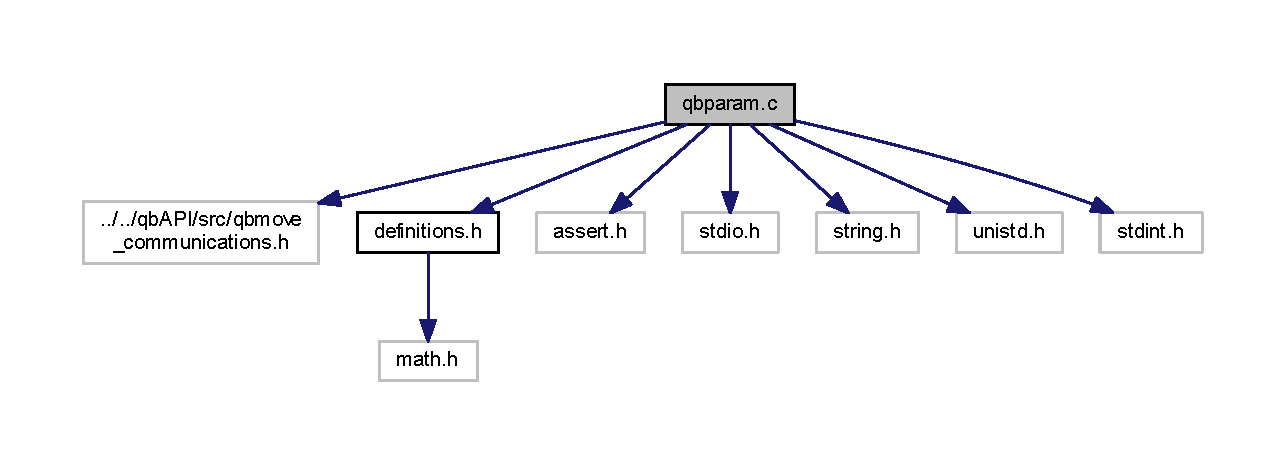
\includegraphics[width=350pt]{qbparam_8c__incl}
\end{center}
\end{figure}
\subsection*{Functions}
\begin{DoxyCompactItemize}
\item 
\mbox{\label{qbparam_8c_a3939d4ef4a0e2be02b1eb9e1994ec985}} 
int {\bfseries port\+\_\+selection} ()
\item 
\mbox{\label{qbparam_8c_abe553924eef0ba8079dc745caf1f348c}} 
int {\bfseries open\+\_\+port} ()
\item 
\mbox{\label{qbparam_8c_a564e2594b1cf22357d72b2e2cf7fdaf3}} 
int {\bfseries init\+Memory} ()
\item 
\mbox{\label{qbparam_8c_af9dce1973196a5934ee5ec20ea417324}} 
void {\bfseries print\+Main\+Menu} ()
\item 
\mbox{\label{qbparam_8c_a9c4b081f1e1ad60def15811c71a936f2}} 
void {\bfseries print\+Version} ()
\item 
\mbox{\label{qbparam_8c_aa78cef14864eb28be4f47d1ebf0e29f1}} 
int {\bfseries calibrate} ()
\item 
int \textbf{ baudrate\+\_\+reader} ()
\item 
\mbox{\label{qbparam_8c_ae66f6b31b5ad750f1fe042a706a4e3d4}} 
int {\bfseries main} ()
\end{DoxyCompactItemize}
\subsection*{Variables}
\begin{DoxyCompactItemize}
\item 
\mbox{\label{qbparam_8c_a3c28322a1b5922f8c61d7cb3723b56b1}} 
char {\bfseries get\+\_\+or\+\_\+set}
\item 
\mbox{\label{qbparam_8c_a92153f4b70cd8ba4e9b502ccff8d28bf}} 
comm\+\_\+settings {\bfseries comm\+\_\+settings\+\_\+t}
\end{DoxyCompactItemize}


\subsection{Detailed Description}
Command line tools file. 

\begin{DoxyAuthor}{Author}
{\itshape Centro \char`\"{}\+E.\+Piaggio\char`\"{}} 
\end{DoxyAuthor}
\begin{DoxyCopyright}{Copyright}
(C) 2012-\/2016 qbrobotics. All rights reserved. 

(C) 2017 Centro \char`\"{}\+E.\+Piaggio\char`\"{}. All rights reserved.
\end{DoxyCopyright}
With this file is possible to get or set firmware parameters. 

\subsection{Function Documentation}
\mbox{\label{qbparam_8c_a872d84bb02f7d8f4617246f0c6d37c43}} 
\index{qbparam.\+c@{qbparam.\+c}!baudrate\+\_\+reader@{baudrate\+\_\+reader}}
\index{baudrate\+\_\+reader@{baudrate\+\_\+reader}!qbparam.\+c@{qbparam.\+c}}
\subsubsection{baudrate\+\_\+reader()}
{\footnotesize\ttfamily int baudrate\+\_\+reader (\begin{DoxyParamCaption}{ }\end{DoxyParamCaption})}

Baudrate functions 
%--- End generated contents ---

% Index
\backmatter
\newpage
\phantomsection
\clearemptydoublepage
\addcontentsline{toc}{chapter}{Index}
\printindex

\end{document}
